\documentclass{article}
\usepackage{graphicx}
\usepackage{fullpage}
\pagestyle{empty} % no header, no page mark
%\usepackage{fontspec}
%\setmainfont{Times New Roman}

\begin{document}

\title{NDN MOG Project Snapshot}
\author{Zening Qu}
\maketitle

\abstract
To be filled.

\tableofcontents
\listoffigures
\listoftables
\newpage

%-------------------------------------------------------------------------------------------------------------------------------------%
% Introduction
%-------------------------------------------------------------------------------------------------------------------------------------%
\section{Introduction}
\label{itro}
Massively Multiplayer Online Games (MMOGs) are gaining research attention these years. The LPP project is an exploration of the design and creation of such games on Named Data Network (NDN). The {consistency}, scalability, availability and security issues of MMOG design are of special interest. As of genre and gameplay, we are interested in creating an Role Playing Game (RPG) inspired by \emph{Le Petit Prince}, which is how this project got its name.

This document is a snapshot of the current progress of the LPP project. It is aimed for the research group to reflect on the finished work and plan the next steps. It contains an in-progress survey of MMOG design issues in the IP world (section \ref{bg}), a brief description of our previous NDN car racing game (section \ref{prew}) and designs of LPP which is our logical next step (section \ref{nstp}). 

%-------------------------------------------------------------------------------------------------------------------------------------%
% Background: MMOG in the IP World
%-------------------------------------------------------------------------------------------------------------------------------------%
\section{Background: MMOG Design Issues in the IP World}
\label{bg}

\subsection{Scale}

%-------------------------------------------------------------------------------------------------------------------------------------%
% Previous Work: about EgalCar
%-------------------------------------------------------------------------------------------------------------------------------------%
\section{Previous Work: Car Racing Game on NDN}
\label{prew}

%-------------------------------------------------------------------------------------------------------------------------------------%
% Introduction
%-------------------------------------------------------------------------------------------------------------------------------------%
\section{Next Step: RPG on NDN}
\label{nstp}

%-------------------------------------------------------------------------------------------------------------------------------------%
\subsection{Namespace Design}

\begin{figure}[htbp]
\begin{center}
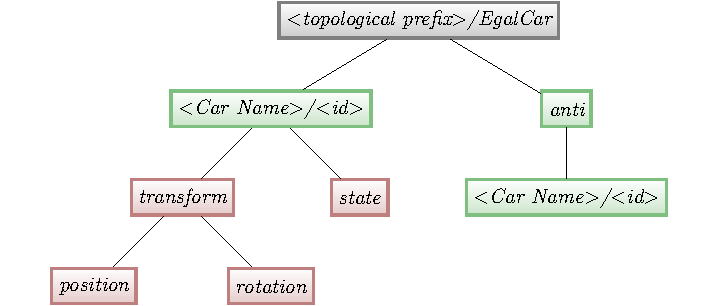
\includegraphics{ObjectTree.pdf}
\caption{Part of LPP's namespace, nodes that contain a ``(sequence number)'' will be explained one by one in this document}
\label{ns}
\end{center}
\end{figure}

\begin{enumerate}
\item \emph{/ndn/ucla.edu/apps/lpp}: the topological prefix of the game
\item \emph{$<$Player ID$>$}: a random number generated in real-time to represent a particular player in the game, this ID is computed in a random manner to (partly) avoid name collisions
\item \emph{$<$Asteroid ID$>$}: a random, real-time number representing a particular asteroid
\item \emph{$<$Seedling ID$>$}: a random, real-time number representing a particular seedling who comes out of a particular asteroid
\item \emph{anti}: this is for asset deletion (publishing an anti-asset corresponds to deleting that particular asset)
\item \emph{.../$<$Player ID$>$/state}: the current state of a particular player; \emph{position} can be used to provide a global view; \emph{experience} can be used to produce a global rank list
\item \emph{.../$<$Asteroid ID$>$/state}: the current state of a particular asteroid, which may contain a name list of all players on that asteroid and things like that
\item \emph{.../$<$Player ID$>$/event}: the action of a particular player
\end{enumerate}

In figure~\ref{ns}, all blue nodes are recognized as \emph{Asset}s, all red nodes \emph{State}s, green ones \emph{Event}s. We will have more documentations about Asset, State, Event in the future. For now it is sufficient to know that these three types of nodes will be synchronized in three different ways.


\end{document}